\title{Perfomancevergleich Mesh Netzwerke}

\team{%
    Raffael Anklin,
    Robin Bobst,
    Cyrill Horath}

%\client{Important Client}

\expert{%
	Jürg M. Stettbacher}

\coaches{%
    Manuel Di Cerbo,
    Matthias Meier}
    

\fssummary{
Die Vernetzung von Sensoren und Aktoren im Low-Power Bereich ist für das Internet der Dinge (IoT) von zentraler Bedeutung.
Immer öfter werden Systeme in diesem Bereich mit sogenannten \textit{Wireless Sensor Networks} realisiert.
Mit typischerweise geringen Latenzzeiten, kleinen Datenraten und geringem Stromverbrauch eignen sich die drei bekanntesten \textit{Low-Power-Mesh-Protokolle} Bluetooth Mesh, Thread und ZigBee perfekt für solche Anwendungen.
Die Eigenschaften sowie Stärken und Schwächen der drei Protokolle werden in diesem Performancevergleich aufgezeigt.
}

\fsgraphics{
\centering
	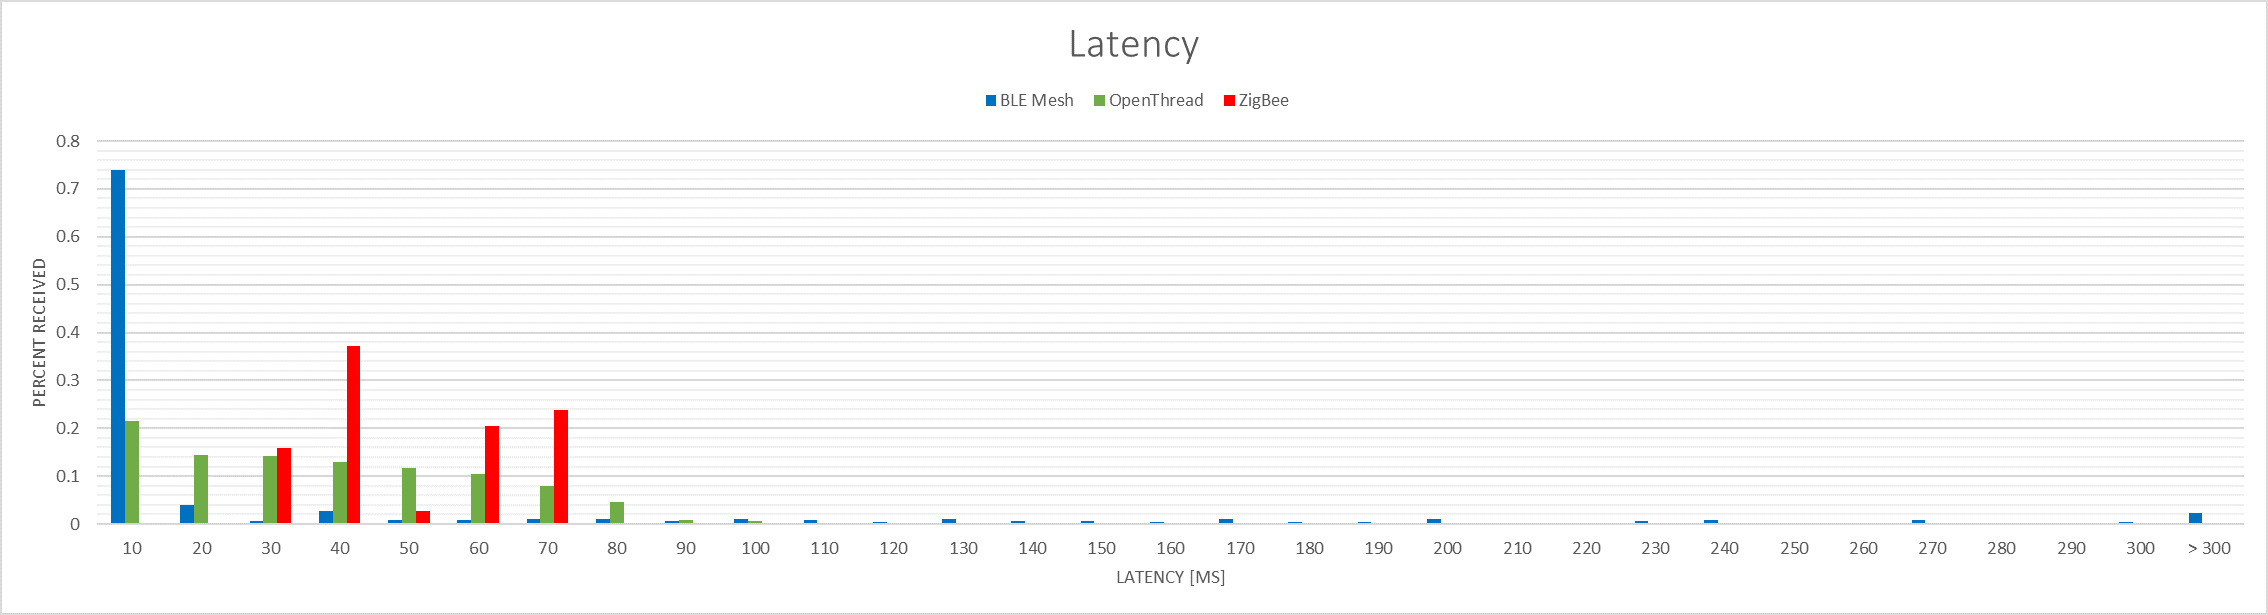
\includegraphics[width=\textwidth]{graphics/Latency_2_Wohnung.png}
    \graphicscaption{Auswertung Messergebnisse Latenzzeiten}
}

\fscontent{
    \section{Konzept}
    Mithilfe der nRF52840-SoC Plattform von Nordic Semiconductor wurde eine einheitliche Plattform geschaffen auf welcher alle drei Protokolle implementiert werden können. Insgesamt 50 Benchmark Nodes die in Gruppen à max. 5 Teilnehmern konfiguriert werden, tauschen Benchmark Pakete aus und generieren damit folgende Daten: Latenzzeit, Durchsatz, Paketverlust und Energieverbrauch.
    Diese Messungen wurden in drei verschiedenen Testaufbauten sowie mit acht unterschiedlichen Messreihen durchgeführt.

%    \newcol
    \section{Umsetzung}
    Die Mesh Nodes für den Benchmark wurden aus nRF52840-Dongle Development Kits aufgebaut welche durch ein Batteriepaket gespeist werden.
    Damit die Plattform für die Messungen tatsächlich einheitlich ist, wurde ein Firmware-Framework entwickelt welches die Steuerungen und Auswertung des Benchmarks übernimmt.
    Dieses kann unabhängig vom Mesh-Protokoll eingesetzt werden da einheitliche Schnittstellen definiert wurden für die Ansteuerung des Protokollstacks.
    
%    \begin{center}
%    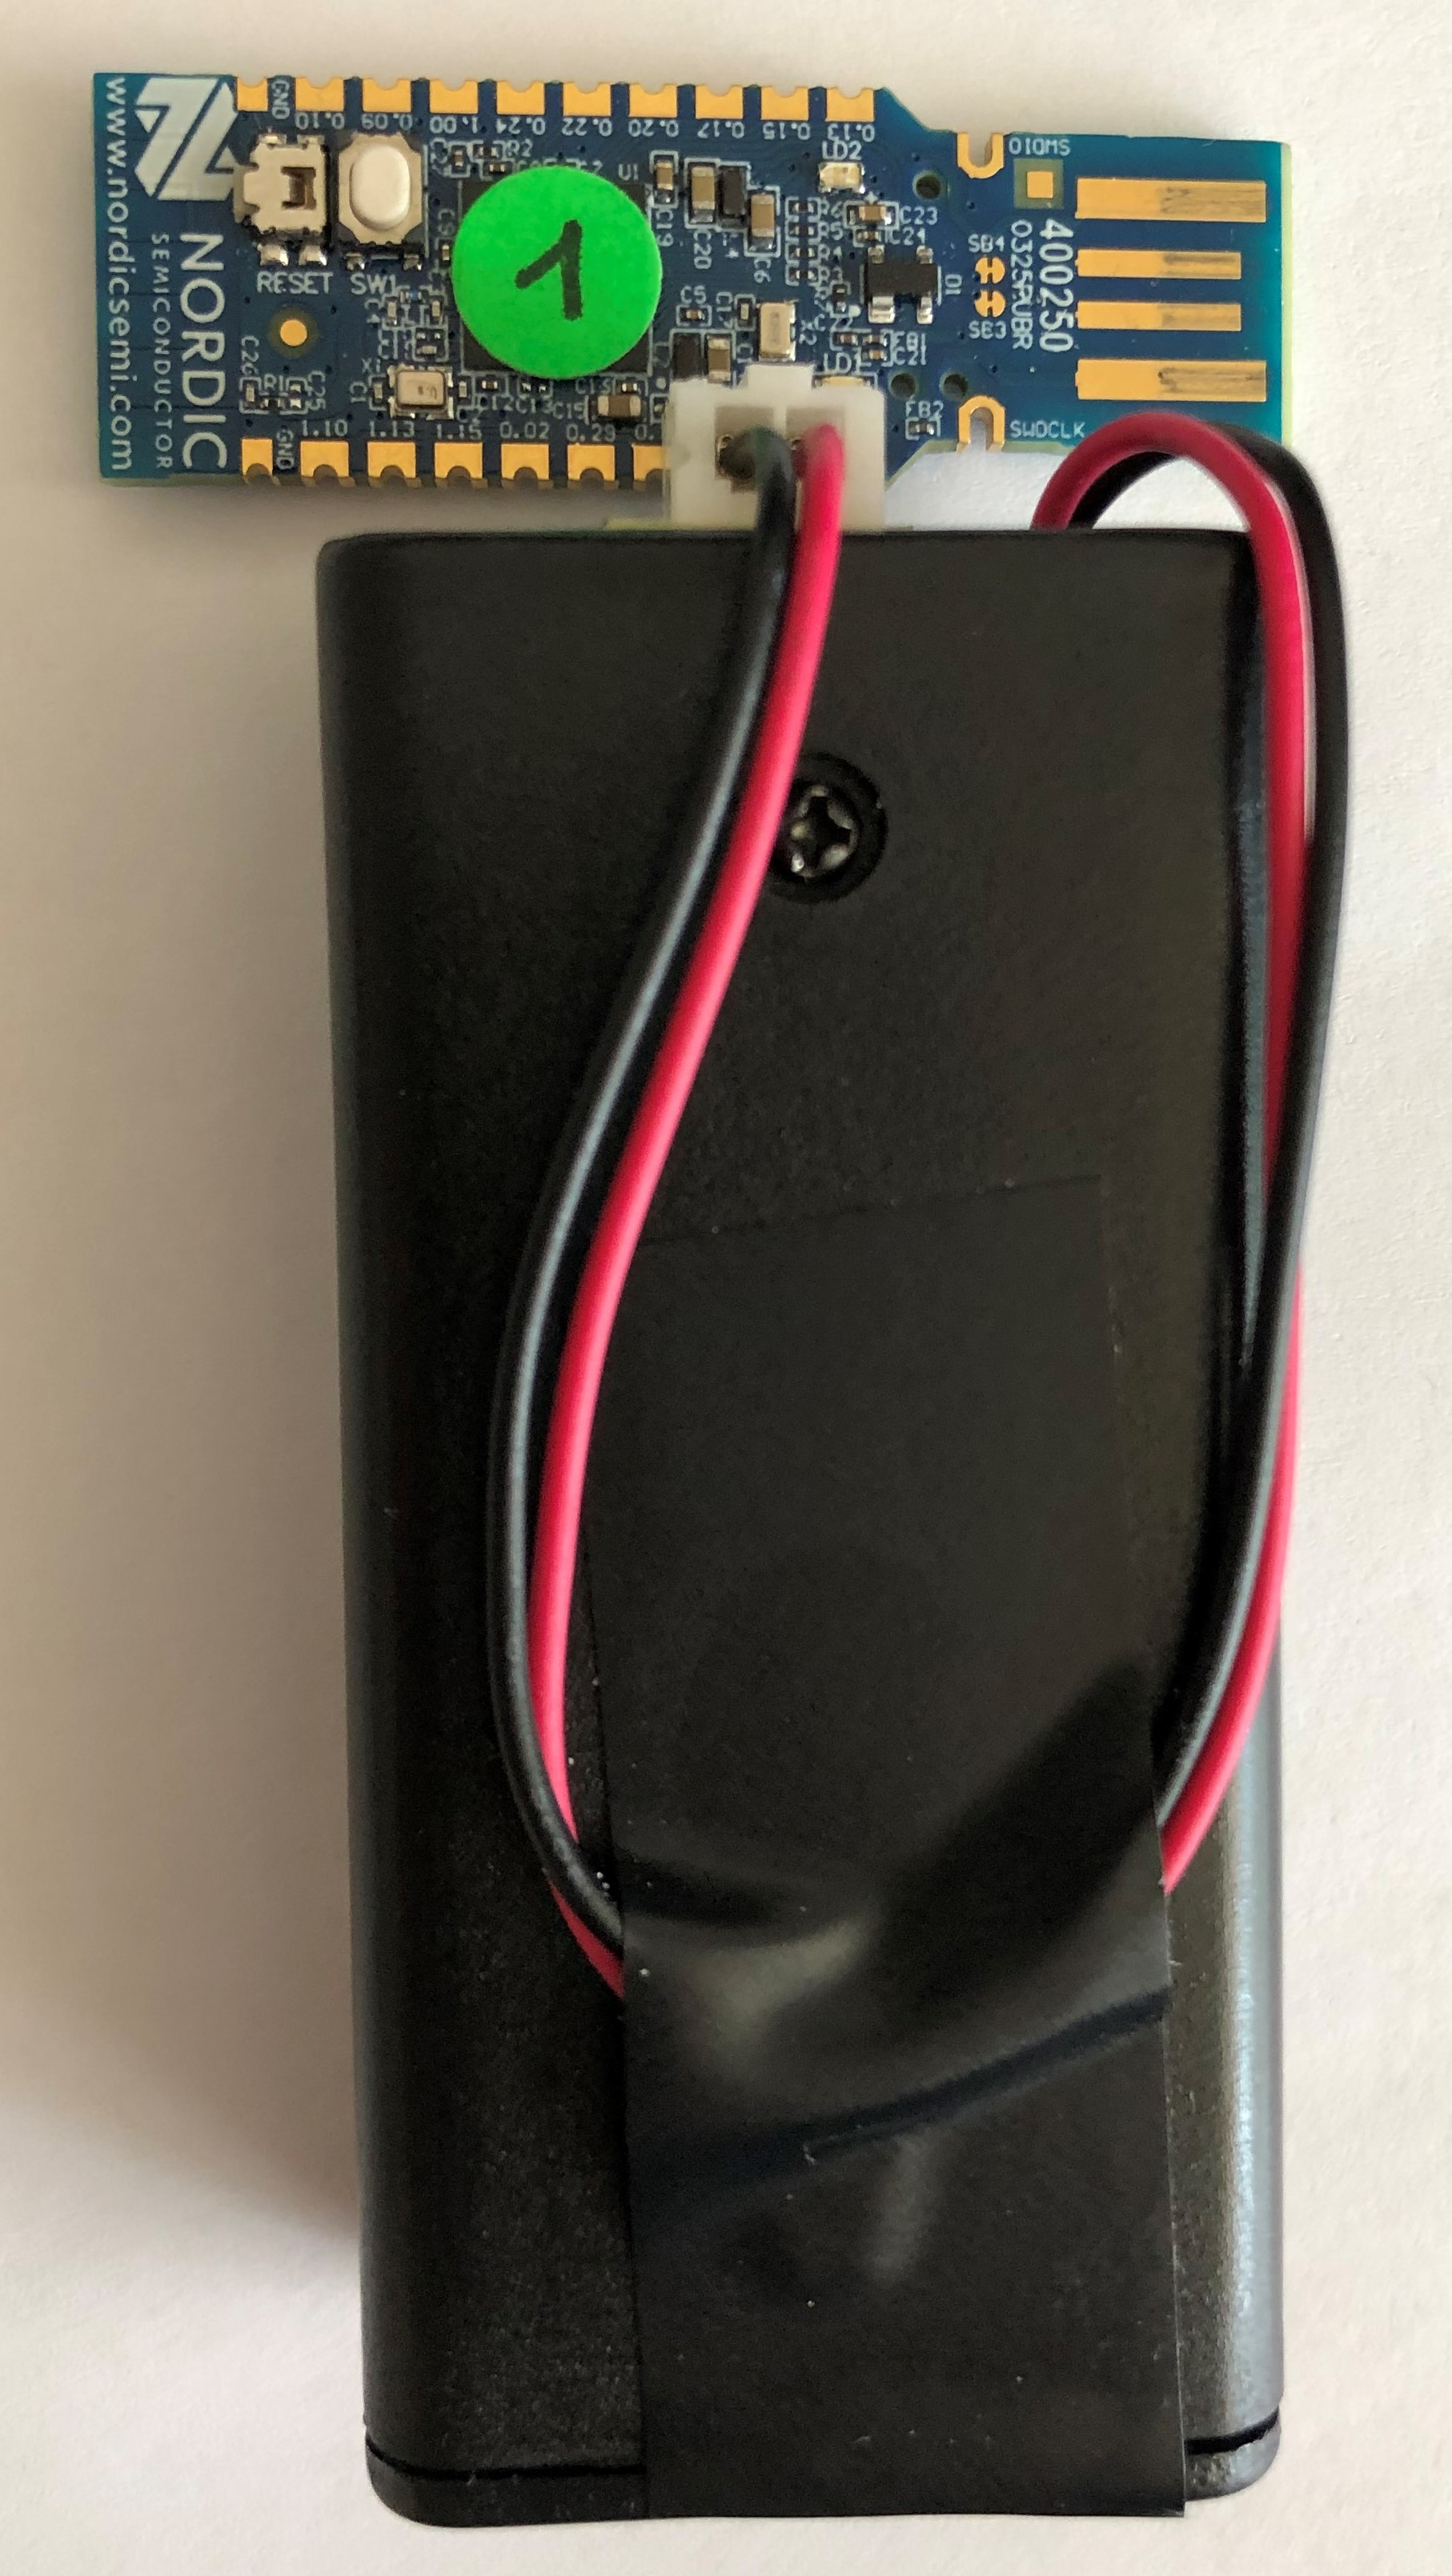
\includegraphics[width=0.4\columnwidth]{graphics/Node_picture.png}
%    \end{center}

%    \newcol
    \section{Resultate}
    Die riesige Flut an Messresultaten wurde mit geeigneten  Tools grafisch aufbereitet und analysiert.
    Ein Beispiel dafür ist die Abbildung oberhalb.
    Darin sind die normalisierten Latenzzeiten der drei Protokolle in Abhängigkeit der Häufigkeit dargestellt.
    Die Grafik zeigt, dass Bluetooth Mesh sehr häufig sehr kleine Latenzzeiten aufweist, jedoch grosse Ausreisser von über 300ms vorhanden sind.
    Diese kommen bei Thread wie auch bei Zigbee nicht vor.
    Thread und ZigBee bauen beide auf dem IEEE 802.15.4 Standard für \textit{Wireless Personal Area Networks (WPAN)} auf und bilden eine geroutetes Mesh Netzwerk. Dies ist auch in der Ergebnissen der Messungen bemerkbar denn sie bewegen sich ungefähr im gleichen Bereich.
	Bluetooth Mesh hingegen nutzt den \textit{Bluetooth Low Energy (BLE)} Standard und ein Flooding Mesh Prinzip.
	Dadurch kann bei hohem Networktraffic nicht die Performance von Thread oder ZigBee erreicht werden.
	Das Gegenteil gilt für geringen Traffic.
	Hier kann Bluetooth Mesh mit dem performanten MAC Layer (BLE) punkten.
    
}

\infobox{Erkenntnisse}{

	 \begin{minipage}{0.69\textwidth}
     \setlength\leftmargini{0.5em}
     \raggedright
     
     Der Sieger des Performancevergleich ist das Thread Protokoll.
     Beim Vergleich der Latenzzeiten wie auch der Paketverlustrate hat es klare Vorteile gegenüber Bluetooth Mesh und auch jene Ergebnisse von Zigbee können übertrumpft werden.
     In der Anwendung muss dieses Ergebnis jedoch relativiert werden. Mit ändernden Bedingungen bezüglich Topologie und Einsatzzweck können Bluetooth Mesh und Zigbee auch grosse Vorteile gegenüber Thread haben.
     Besonders das Flooding Mesh Prinzip bei Bluetooth Mesh und der standardisierte Application Layer bei Zigbee haben je nach Anwendung positive Eigenschaften. 
     	
%	Einen klaren Sieger kann aus dem Performancevergleich nicht bestimmt werden. Jedes der drei Protokolle hat je nach Anwendung Vor- und auch Nachteile.
%	Da Thread IPv6 für die Adressierung einsetzt ist es sehr einfach in IoT Anwendungen integrierbar. Das macht den Stack sicherlich zu jenem der in Zukunft die Anwendungen dominieren wird.
    \end{minipage}
    \hfill
    \begin{minipage}{0.3\textwidth}
        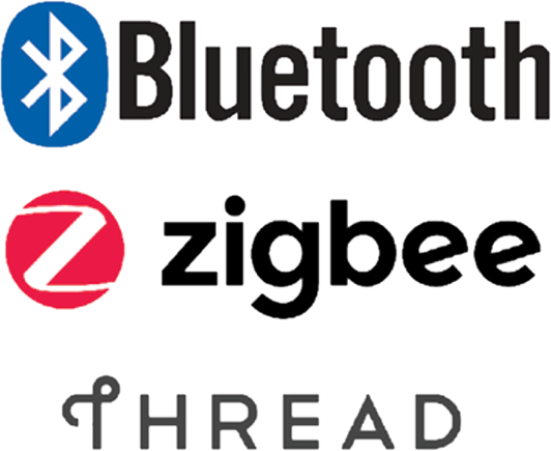
\includegraphics[width=\textwidth]{graphics/Protocols.png}
        \graphicssource{circuitcellar.com}
    \end{minipage}
}
